\chapter{Validación}

La estrategia combina pruebas de integración de API y pruebas de componentes/rutas de frontend. Las primeras arrancan la aplicación completa con \texttt{WebApplicationFactory} y sustituyen solo PostgreSQL por una base en memoria aislada. Las segundas simulan la API y manipulan la interfaz como lo haría una persona usuaria.

\begin{table}[htbp]
\centering
\caption{Pruebas automatizadas del Sprint 1}
\begin{tabular}{p{6.2cm}p{2cm}p{2.5cm}}
\hline Comportamiento & Capa & Resultado \\ \hline
Primer administrador y hash de contraseña & Backend & Correcto \\
Bloqueo de un segundo bootstrap & Backend & Correcto \\
Login válido, erróneo y usuario inactivo & Backend & Correcto \\
Rutas protegidas 401 y 403 & Backend & Correcto \\
Contrato de validación & Backend & Correcto \\
Redirección sin sesión & Frontend & Correcto \\
Login, persistencia y error visible & Frontend & Correcto \\
Navegación adaptada al rol administrador & Frontend & Correcto \\
\hline
\end{tabular}
\end{table}

La ejecución local al cierre del incremento produjo dieciséis pruebas backend, organizadas por servicio y controlador, y cuatro frontend correctas, además de build de producción de ambos proyectos. La CI repite las mismas comprobaciones y valida la migración sobre PostgreSQL 16. Las pruebas funcionales de sistema crecerán con cada flujo y se consolidarán en el Sprint 7.

\clearpage
\begin{table}[htbp]
\centering
\caption{Validación acumulada de los Sprints 2 y 3}
\begin{tabular}{p{5.8cm}p{2.4cm}p{2.5cm}}
\hline Comportamiento & Capa & Resultado \\ \hline
CRUD y baja lógica de los tres catálogos & Backend/Frontend & Correcto \\
Unicidad y reutilización tras baja & Backend & Correcto \\
Alta, consulta y edición de envíos & Backend/Frontend & Correcto \\
Normalización UTC de formatos Z, sin zona y con offset & Backend & Correcto \\
Regla de fechas y errores por campo & Backend/Frontend & Correcto \\
Filtros combinables y paginación estable & Backend/Frontend & Correcto \\
Cliente activo y conservación del vínculo histórico & Backend & Correcto \\
\hline
\end{tabular}
\end{table}

Tras el Sprint 2 se ejecutaban 29 pruebas backend y 7 frontend. El Sprint 3 añadió 16 y 6 respectivamente, elevando el total a 45 pruebas backend y 13 frontend, todas correctas junto con el lint y las compilaciones de producción.

\begin{table}[htbp]
\centering
\caption{Validación del Sprint 4}
\begin{tabular}{p{6.1cm}p{2.2cm}p{2.3cm}}
\hline Comportamiento & Capa & Resultado \\ \hline
Asignación conjunta y retirada idempotente & Backend/Frontend & Correcto \\
Recursos activos y exclusión del propio envío & Backend & Correcto \\
Anti-doble-reserva en estados abiertos & Backend/Sistema & Correcto \\
Aviso no bloqueante de capacidad & Backend/Frontend & Correcto \\
Transiciones válidas, inválidas y terminales & Backend/Frontend & Correcto \\
Sellado UTC de recogida y entrega reales & Backend/PostgreSQL & Correcto \\
Proyección de matrícula y conductor en PostgreSQL & Integración & Correcto \\
\hline
\end{tabular}
\end{table}

El cierre del Sprint 4 elevó el total a 74 pruebas backend y 19 frontend. Además de las suites, se ejecutó el flujo integrado mediante Nginx, API y PostgreSQL 16: se verificaron la migración, las proyecciones SQL, el aviso de capacidad, el conflicto que identifica el envío ocupante y el bloqueo visual de un estado final. La prueba en navegador descubrió además un caso de fecha inválida que podía dejar el formulario pendiente; se corrigió y quedó cubierto por una prueba de regresión.

\begin{figure}[htbp]
\centering
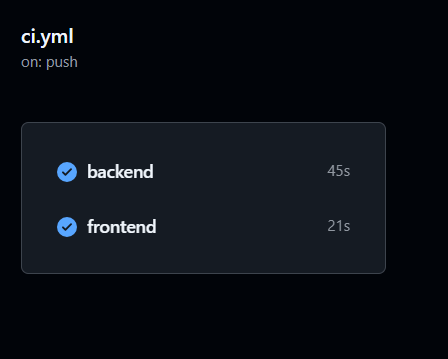
\includegraphics[width=0.4\textwidth]{imaxes/ci-verde}
\caption{Ejecución de la integración continua en verde tras publicar la rama}
\label{fig:ci-verde}
\end{figure}
